\documentclass{report}

\usepackage{float}
\documentclass[12pt]{article}
\usepackage{array}
\usepackage{color}
\usepackage{amsthm}
\usepackage{eufrak}
\usepackage{lipsum}
\usepackage{pifont}
\usepackage{yfonts}
\usepackage{amsmath}
\usepackage{amssymb}
\usepackage{ccfonts}
\usepackage{comment} \usepackage{amsfonts}
\usepackage{fancyhdr}
\usepackage{graphicx}
\usepackage{listings}
\usepackage{mathrsfs}
\usepackage{setspace}
\usepackage{textcomp}
\usepackage{blindtext}
\usepackage{enumerate}
\usepackage{microtype}
\usepackage{xfakebold}
\usepackage{kantlipsum}
%\usepackage{draftwatermark}
\usepackage[spanish]{babel}
\usepackage[margin=1.5cm, top=2cm, bottom=2cm]{geometry}
\usepackage[framemethod=tikz]{mdframed}
\usepackage[colorlinks=true,citecolor=blue,linkcolor=red,urlcolor=magenta]{hyperref}

%//////////////////////////////////////////////////////
% Watermark configuration
%//////////////////////////////////////////////////////
%\SetWatermarkScale{4}
%\SetWatermarkColor{black}
%\SetWatermarkLightness{0.95}
%\SetWatermarkText{\texttt{Watermark}}

%//////////////////////////////////////////////////////
% Frame configuration
%//////////////////////////////////////////////////////
\newmdenv[tikzsetting={draw=gray,fill=white,fill opacity=0},backgroundcolor=none]{Frame}

%//////////////////////////////////////////////////////
% Font style configuration
%//////////////////////////////////////////////////////
\renewcommand{\familydefault}{\ttdefault}
\renewcommand{\rmdefault}{tt}

%//////////////////////////////////////////////////////
% Bold configuration
%//////////////////////////////////////////////////////
\newcommand{\fbseries}{\unskip\setBold\aftergroup\unsetBold\aftergroup\ignorespaces}
\makeatletter
\newcommand{\setBoldness}[1]{\def\fake@bold{#1}}
\makeatother

%//////////////////////////////////////////////////////
% Default font configuration
%//////////////////////////////////////////////////////
\DeclareFontFamily{\encodingdefault}{\ttdefault}{%
  \hyphenchar\font=\defaulthyphenchar
  \fontdimen2\font=0.33333em
  \fontdimen3\font=0.16667em
  \fontdimen4\font=0.11111em
  \fontdimen7\font=0.11111em}


%From M275 "Topology" at SJSU
\newcommand{\id}{\mathrm{id}}
\newcommand{\taking}[1]{\xrightarrow{#1}}
\newcommand{\inv}{^{-1}}

%From M170 "Introduction to Graph Theory" at SJSU
\DeclareMathOperator{\diam}{diam}
\DeclareMathOperator{\ord}{ord}
\newcommand{\defeq}{\overset{\mathrm{def}}{=}}

%From the USAMO .tex files
\newcommand{\ts}{\textsuperscript}
\newcommand{\dg}{^\circ}
\newcommand{\ii}{\item}

% % From Math 55 and Math 145 at Harvard
% \newenvironment{subproof}[1][Proof]{%
% \begin{proof}[#1] \renewcommand{\qedsymbol}{$\blacksquare$}}%
% {\end{proof}}

\newcommand{\liff}{\leftrightarrow}
\newcommand{\lthen}{\rightarrow}
\newcommand{\opname}{\operatorname}
\newcommand{\surjto}{\twoheadrightarrow}
\newcommand{\injto}{\hookrightarrow}
\newcommand{\On}{\mathrm{On}} % ordinals
\DeclareMathOperator{\img}{im} % Image
\DeclareMathOperator{\Img}{Im} % Image
\DeclareMathOperator{\coker}{coker} % Cokernel
\DeclareMathOperator{\Coker}{Coker} % Cokernel
\DeclareMathOperator{\Ker}{Ker} % Kernel
\DeclareMathOperator{\rank}{rank}
\DeclareMathOperator{\Spec}{Spec} % spectrum
\DeclareMathOperator{\Tr}{Tr} % trace
\DeclareMathOperator{\pr}{pr} % projection
\DeclareMathOperator{\ext}{ext} % extension
\DeclareMathOperator{\pred}{pred} % predecessor
\DeclareMathOperator{\dom}{dom} % domain
\DeclareMathOperator{\ran}{ran} % range
\DeclareMathOperator{\Hom}{Hom} % homomorphism
\DeclareMathOperator{\Mor}{Mor} % morphisms
\DeclareMathOperator{\End}{End} % endomorphism

\newcommand{\eps}{\epsilon}
\newcommand{\veps}{\varepsilon}
\newcommand{\ol}{\overline}
\newcommand{\ul}{\underline}
\newcommand{\wt}{\widetilde}
\newcommand{\wh}{\widehat}
\newcommand{\vocab}[1]{\textbf{\color{blue} #1}}
\providecommand{\half}{\frac{1}{2}}
\newcommand{\dang}{\measuredangle} %% Directed angle
\newcommand{\ray}[1]{\overrightarrow{#1}}
\newcommand{\seg}[1]{\overline{#1}}
\newcommand{\arc}[1]{\wideparen{#1}}
\DeclareMathOperator{\cis}{cis}
\DeclareMathOperator*{\lcm}{lcm}
\DeclareMathOperator*{\argmin}{arg min}
\DeclareMathOperator*{\argmax}{arg max}
\newcommand{\cycsum}{\sum_{\mathrm{cyc}}}
\newcommand{\symsum}{\sum_{\mathrm{sym}}}
\newcommand{\cycprod}{\prod_{\mathrm{cyc}}}
\newcommand{\symprod}{\prod_{\mathrm{sym}}}
\newcommand{\Qed}{\begin{flushright}\qed\end{flushright}}
\newcommand{\parinn}{\setlength{\parindent}{1cm}}
\newcommand{\parinf}{\setlength{\parindent}{0cm}}
% \newcommand{\norm}{\|\cdot\|}
\newcommand{\inorm}{\norm_{\infty}}
\newcommand{\opensets}{\{V_{\alpha}\}_{\alpha\in I}}
\newcommand{\oset}{V_{\alpha}}
\newcommand{\opset}[1]{V_{\alpha_{#1}}}
\newcommand{\lub}{\text{lub}}
\newcommand{\del}[2]{\frac{\partial #1}{\partial #2}}
\newcommand{\Del}[3]{\frac{\partial^{#1} #2}{\partial^{#1} #3}}
\newcommand{\deld}[2]{\dfrac{\partial #1}{\partial #2}}
\newcommand{\Deld}[3]{\dfrac{\partial^{#1} #2}{\partial^{#1} #3}}
\newcommand{\lm}{\lambda}
\newcommand{\uin}{\mathbin{\rotatebox[origin=c]{90}{$\in$}}}
\newcommand{\usubset}{\mathbin{\rotatebox[origin=c]{90}{$\subset$}}}
\newcommand{\lt}{\left}
\newcommand{\rt}{\right}
\newcommand{\paren}[1]{\left(#1\right)}
\newcommand{\bs}[1]{\boldsymbol{#1}}
\newcommand{\exs}{\exists}
\newcommand{\st}{\strut}
\newcommand{\dps}[1]{\displaystyle{#1}}

\newcommand{\sol}{\setlength{\parindent}{0cm}\textbf{\textit{Solution:}}\setlength{\parindent}{1cm} }
\newcommand{\solve}[1]{\setlength{\parindent}{0cm}\textbf{\textit{Solution: }}\setlength{\parindent}{1cm}#1 \Qed}

% Things Lie
\newcommand{\kb}{\mathfrak b}
\newcommand{\kg}{\mathfrak g}
\newcommand{\kh}{\mathfrak h}
\newcommand{\kn}{\mathfrak n}
\newcommand{\ku}{\mathfrak u}
\newcommand{\kz}{\mathfrak z}
\DeclareMathOperator{\Ext}{Ext} % Ext functor
\DeclareMathOperator{\Tor}{Tor} % Tor functor
\newcommand{\gl}{\opname{\mathfrak{gl}}} % frak gl group
\renewcommand{\sl}{\opname{\mathfrak{sl}}} % frak sl group chktex 6

% More script letters etc.
\newcommand{\SA}{\mathcal A}
\newcommand{\SB}{\mathcal B}
\newcommand{\SC}{\mathcal C}
\newcommand{\SF}{\mathcal F}
\newcommand{\SG}{\mathcal G}
\newcommand{\SH}{\mathcal H}
\newcommand{\OO}{\mathcal O}

\newcommand{\SCA}{\mathscr A}
\newcommand{\SCB}{\mathscr B}
\newcommand{\SCC}{\mathscr C}
\newcommand{\SCD}{\mathscr D}
\newcommand{\SCE}{\mathscr E}
\newcommand{\SCF}{\mathscr F}
\newcommand{\SCG}{\mathscr G}
\newcommand{\SCH}{\mathscr H}

% Mathfrak primes
\newcommand{\km}{\mathfrak m}
\newcommand{\kp}{\mathfrak p}
\newcommand{\kq}{\mathfrak q}

% number sets
\newcommand{\RR}[1][]{\ensuremath{\ifstrempty{#1}{\mathbb{R}}{\mathbb{R}^{#1}}}}
\newcommand{\NN}[1][]{\ensuremath{\ifstrempty{#1}{\mathbb{N}}{\mathbb{N}^{#1}}}}
\newcommand{\ZZ}[1][]{\ensuremath{\ifstrempty{#1}{\mathbb{Z}}{\mathbb{Z}^{#1}}}}
\newcommand{\QQ}[1][]{\ensuremath{\ifstrempty{#1}{\mathbb{Q}}{\mathbb{Q}^{#1}}}}
\newcommand{\CC}[1][]{\ensuremath{\ifstrempty{#1}{\mathbb{C}}{\mathbb{C}^{#1}}}}
\newcommand{\PP}[1][]{\ensuremath{\ifstrempty{#1}{\mathbb{P}}{\mathbb{P}^{#1}}}}
\newcommand{\HH}[1][]{\ensuremath{\ifstrempty{#1}{\mathbb{H}}{\mathbb{H}^{#1}}}}
\newcommand{\FF}[1][]{\ensuremath{\ifstrempty{#1}{\mathbb{F}}{\mathbb{F}^{#1}}}}
% expected value
\newcommand{\EE}{\ensuremath{\mathbb{E}}}
\newcommand{\charin}{\text{ char }}
\DeclareMathOperator{\sign}{sign}
\DeclareMathOperator{\Aut}{Aut}
\DeclareMathOperator{\Inn}{Inn}
\DeclareMathOperator{\Syl}{Syl}
\DeclareMathOperator{\Gal}{Gal}
\DeclareMathOperator{\GL}{GL} % General linear group
\DeclareMathOperator{\SL}{SL} % Special linear group

%---------------------------------------
% BlackBoard Math Fonts :-
%---------------------------------------

%Captital Letters
\newcommand{\bbA}{\mathbb{A}}	\newcommand{\bbB}{\mathbb{B}}
\newcommand{\bbC}{\mathbb{C}}	\newcommand{\bbD}{\mathbb{D}}
\newcommand{\bbE}{\mathbb{E}}	\newcommand{\bbF}{\mathbb{F}}
\newcommand{\bbG}{\mathbb{G}}	\newcommand{\bbH}{\mathbb{H}}
\newcommand{\bbI}{\mathbb{I}}	\newcommand{\bbJ}{\mathbb{J}}
\newcommand{\bbK}{\mathbb{K}}	\newcommand{\bbL}{\mathbb{L}}
\newcommand{\bbM}{\mathbb{M}}	\newcommand{\bbN}{\mathbb{N}}
\newcommand{\bbO}{\mathbb{O}}	\newcommand{\bbP}{\mathbb{P}}
\newcommand{\bbQ}{\mathbb{Q}}	\newcommand{\bbR}{\mathbb{R}}
\newcommand{\bbS}{\mathbb{S}}	\newcommand{\bbT}{\mathbb{T}}
\newcommand{\bbU}{\mathbb{U}}	\newcommand{\bbV}{\mathbb{V}}
\newcommand{\bbW}{\mathbb{W}}	\newcommand{\bbX}{\mathbb{X}}
\newcommand{\bbY}{\mathbb{Y}}	\newcommand{\bbZ}{\mathbb{Z}}

%---------------------------------------
% MathCal Fonts :-
%---------------------------------------

%Captital Letters
\newcommand{\mcA}{\mathcal{A}}	\newcommand{\mcB}{\mathcal{B}}
\newcommand{\mcC}{\mathcal{C}}	\newcommand{\mcD}{\mathcal{D}}
\newcommand{\mcE}{\mathcal{E}}	\newcommand{\mcF}{\mathcal{F}}
\newcommand{\mcG}{\mathcal{G}}	\newcommand{\mcH}{\mathcal{H}}
\newcommand{\mcI}{\mathcal{I}}	\newcommand{\mcJ}{\mathcal{J}}
\newcommand{\mcK}{\mathcal{K}}	\newcommand{\mcL}{\mathcal{L}}
\newcommand{\mcM}{\mathcal{M}}	\newcommand{\mcN}{\mathcal{N}}
\newcommand{\mcO}{\mathcal{O}}	\newcommand{\mcP}{\mathcal{P}}
\newcommand{\mcQ}{\mathcal{Q}}	\newcommand{\mcR}{\mathcal{R}}
\newcommand{\mcS}{\mathcal{S}}	\newcommand{\mcT}{\mathcal{T}}
\newcommand{\mcU}{\mathcal{U}}	\newcommand{\mcV}{\mathcal{V}}
\newcommand{\mcW}{\mathcal{W}}	\newcommand{\mcX}{\mathcal{X}}
\newcommand{\mcY}{\mathcal{Y}}	\newcommand{\mcZ}{\mathcal{Z}}


%---------------------------------------
% Bold Math Fonts :-
%---------------------------------------

%Captital Letters
\newcommand{\bmA}{\boldsymbol{A}}	\newcommand{\bmB}{\boldsymbol{B}}
\newcommand{\bmC}{\boldsymbol{C}}	\newcommand{\bmD}{\boldsymbol{D}}
\newcommand{\bmE}{\boldsymbol{E}}	\newcommand{\bmF}{\boldsymbol{F}}
\newcommand{\bmG}{\boldsymbol{G}}	\newcommand{\bmH}{\boldsymbol{H}}
\newcommand{\bmI}{\boldsymbol{I}}	\newcommand{\bmJ}{\boldsymbol{J}}
\newcommand{\bmK}{\boldsymbol{K}}	\newcommand{\bmL}{\boldsymbol{L}}
\newcommand{\bmM}{\boldsymbol{M}}	\newcommand{\bmN}{\boldsymbol{N}}
\newcommand{\bmO}{\boldsymbol{O}}	\newcommand{\bmP}{\boldsymbol{P}}
\newcommand{\bmQ}{\boldsymbol{Q}}	\newcommand{\bmR}{\boldsymbol{R}}
\newcommand{\bmS}{\boldsymbol{S}}	\newcommand{\bmT}{\boldsymbol{T}}
\newcommand{\bmU}{\boldsymbol{U}}	\newcommand{\bmV}{\boldsymbol{V}}
\newcommand{\bmW}{\boldsymbol{W}}	\newcommand{\bmX}{\boldsymbol{X}}
\newcommand{\bmY}{\boldsymbol{Y}}	\newcommand{\bmZ}{\boldsymbol{Z}}
%Small Letters
\newcommand{\bma}{\boldsymbol{a}}	\newcommand{\bmb}{\boldsymbol{b}}
\newcommand{\bmc}{\boldsymbol{c}}	\newcommand{\bmd}{\boldsymbol{d}}
\newcommand{\bme}{\boldsymbol{e}}	\newcommand{\bmf}{\boldsymbol{f}}
\newcommand{\bmg}{\boldsymbol{g}}	\newcommand{\bmh}{\boldsymbol{h}}
\newcommand{\bmi}{\boldsymbol{i}}	\newcommand{\bmj}{\boldsymbol{j}}
\newcommand{\bmk}{\boldsymbol{k}}	\newcommand{\bml}{\boldsymbol{l}}
\newcommand{\bmm}{\boldsymbol{m}}	\newcommand{\bmn}{\boldsymbol{n}}
\newcommand{\bmo}{\boldsymbol{o}}	\newcommand{\bmp}{\boldsymbol{p}}
\newcommand{\bmq}{\boldsymbol{q}}	\newcommand{\bmr}{\boldsymbol{r}}
\newcommand{\bms}{\boldsymbol{s}}	\newcommand{\bmt}{\boldsymbol{t}}
\newcommand{\bmu}{\boldsymbol{u}}	\newcommand{\bmv}{\boldsymbol{v}}
\newcommand{\bmw}{\boldsymbol{w}}	\newcommand{\bmx}{\boldsymbol{x}}
\newcommand{\bmy}{\boldsymbol{y}}	\newcommand{\bmz}{\boldsymbol{z}}

%---------------------------------------
% Scr Math Fonts :-
%---------------------------------------

\newcommand{\sA}{{\mathscr{A}}}   \newcommand{\sB}{{\mathscr{B}}}
\newcommand{\sC}{{\mathscr{C}}}   \newcommand{\sD}{{\mathscr{D}}}
\newcommand{\sE}{{\mathscr{E}}}   \newcommand{\sF}{{\mathscr{F}}}
\newcommand{\sG}{{\mathscr{G}}}   \newcommand{\sH}{{\mathscr{H}}}
\newcommand{\sI}{{\mathscr{I}}}   \newcommand{\sJ}{{\mathscr{J}}}
\newcommand{\sK}{{\mathscr{K}}}   \newcommand{\sL}{{\mathscr{L}}}
\newcommand{\sM}{{\mathscr{M}}}   \newcommand{\sN}{{\mathscr{N}}}
\newcommand{\sO}{{\mathscr{O}}}   \newcommand{\sP}{{\mathscr{P}}}
\newcommand{\sQ}{{\mathscr{Q}}}   \newcommand{\sR}{{\mathscr{R}}}
\newcommand{\sS}{{\mathscr{S}}}   \newcommand{\sT}{{\mathscr{T}}}
\newcommand{\sU}{{\mathscr{U}}}   \newcommand{\sV}{{\mathscr{V}}}
\newcommand{\sW}{{\mathscr{W}}}   \newcommand{\sX}{{\mathscr{X}}}
\newcommand{\sY}{{\mathscr{Y}}}   \newcommand{\sZ}{{\mathscr{Z}}}


%---------------------------------------
% Math Fraktur Font
%---------------------------------------

%Captital Letters
\newcommand{\mfA}{\mathfrak{A}}	\newcommand{\mfB}{\mathfrak{B}}
\newcommand{\mfC}{\mathfrak{C}}	\newcommand{\mfD}{\mathfrak{D}}
\newcommand{\mfE}{\mathfrak{E}}	\newcommand{\mfF}{\mathfrak{F}}
\newcommand{\mfG}{\mathfrak{G}}	\newcommand{\mfH}{\mathfrak{H}}
\newcommand{\mfI}{\mathfrak{I}}	\newcommand{\mfJ}{\mathfrak{J}}
\newcommand{\mfK}{\mathfrak{K}}	\newcommand{\mfL}{\mathfrak{L}}
\newcommand{\mfM}{\mathfrak{M}}	\newcommand{\mfN}{\mathfrak{N}}
\newcommand{\mfO}{\mathfrak{O}}	\newcommand{\mfP}{\mathfrak{P}}
\newcommand{\mfQ}{\mathfrak{Q}}	\newcommand{\mfR}{\mathfrak{R}}
\newcommand{\mfS}{\mathfrak{S}}	\newcommand{\mfT}{\mathfrak{T}}
\newcommand{\mfU}{\mathfrak{U}}	\newcommand{\mfV}{\mathfrak{V}}
\newcommand{\mfW}{\mathfrak{W}}	\newcommand{\mfX}{\mathfrak{X}}
\newcommand{\mfY}{\mathfrak{Y}}	\newcommand{\mfZ}{\mathfrak{Z}}
%Small Letters
\newcommand{\mfa}{\mathfrak{a}}	\newcommand{\mfb}{\mathfrak{b}}
\newcommand{\mfc}{\mathfrak{c}}	\newcommand{\mfd}{\mathfrak{d}}
\newcommand{\mfe}{\mathfrak{e}}	\newcommand{\mff}{\mathfrak{f}}
\newcommand{\mfg}{\mathfrak{g}}	\newcommand{\mfh}{\mathfrak{h}}
\newcommand{\mfi}{\mathfrak{i}}	\newcommand{\mfj}{\mathfrak{j}}
\newcommand{\mfk}{\mathfrak{k}}	\newcommand{\mfl}{\mathfrak{l}}
\newcommand{\mfm}{\mathfrak{m}}	\newcommand{\mfn}{\mathfrak{n}}
\newcommand{\mfo}{\mathfrak{o}}	\newcommand{\mfp}{\mathfrak{p}}
\newcommand{\mfq}{\mathfrak{q}}	\newcommand{\mfr}{\mathfrak{r}}
\newcommand{\mfs}{\mathfrak{s}}	\newcommand{\mft}{\mathfrak{t}}
\newcommand{\mfu}{\mathfrak{u}}	\newcommand{\mfv}{\mathfrak{v}}
\newcommand{\mfw}{\mathfrak{w}}	\newcommand{\mfx}{\mathfrak{x}}
\newcommand{\mfy}{\mathfrak{y}}	\newcommand{\mfz}{\mathfrak{z}}


\title{\Huge{Métodos Matemáticos}\\Tarea 2}
\author{\huge{Sergio Montoya Ramírez}}
\date{}

\begin{document}

\maketitle
\newpage% or \cleardoublepage
% \pdfbookmark[<level>]{<title>}{<dest>}
\pdfbookmark[section]{\contentsname}{toc}
\tableofcontents
\pagebreak

\chapter{Pregunta 1: 11.7.1}

\qs{Pregunta 11.7.1}{
  Determine la naturaleza de las singularidades para cada una de las siguientes funciones y evalué el residuo $\left( a > 0 \right) $
  \begin{multicols}{2}
    \begin{enumerate}
      \item $\frac{1}{z^2 + a^2}$.
      \item $\frac{1}{\left( z^2 + a^2 \right)^2}$.
      \item $\frac{z^2}{\left( z^2 + a^2 \right)^2}$.
      \item $\frac{\sin\left( \frac{1}{z} \right) }{z^2 + a^2}$.
      \item $\frac{ze^{+iz}}{z^2 + a^2}$.
      \item $\frac{ze^{+iz}}{z^2 - a^2}$.
      \item $\frac{e^{+iz}}{z^2 - a^2}$.
      \item $\frac{z^{-k}}{z + 1}$. $0<k<1$.
    \end{enumerate}
  \end{multicols}
}

\begin{enumerate}
  \item $\frac{1}{z^2 + a^2} = \frac{1}{\left( z - ia \right) \left( z + ia \right) }$. Por lo tanto, tiene dos polos simples $\left\{ ia, -ia \right\} $. Ademas, los residuos serian $\left\{ \frac{1}{2ia}, - \frac{1}{2ia} \right\} $

  \item $\frac{1}{\left( z^2 + a^2 \right)^2} = \frac{1}{\left( z - ia \right)^2 \left( z + ia \right)^2}	$. De manera parecida al anterior, estos son dos polos pero esta vez de segundo orden. Por lo tanto, sus residuos serian $\left\{ \frac{1}{\left( 4a^{3}i \right) } , - \frac{1}{4a^{3}i}\right\} $
  \item $\frac{z^2}{\left( z^2 + a^2 \right)^2}$.

    Ahora con este note que: \[
      \frac{z^2}{\left( z^2 + a^2 \right)^2} = \frac{z^2}{\left( z - ia \right)^2\left( z + ia \right)^2}
      .\] por lo tanto sus polos son los mismo $\left\{ ia, -ia \right\} $. Sin embargo ahora sus residuos tienen encima un $z^2$ por lo que el resultado seria $\left\{ -\frac{1}{4ai}, \frac{1}{4ai} \right\} $
  \item $\frac{\sin\left( \frac{1}{z} \right) }{z^2 + a^2}$.

    En este caso tenemos un resultado muy similar al del inicio donde tenemos dos polos simples en $\left\{ ia, -ia \right\} $. En este caso al evaluar nos queda:
    \begin{align*}
      \frac{\sin\left( \frac{1}{ai} \right) }{2ai} &= -\frac{\sin\left( -\frac{i}{a} \right)i }{2a} \\
      &= -\frac{\sinh\left( \frac{1}{a} \right) }{2a} \\
    .\end{align*}
  \item $\frac{ze^{+iz}}{z^2 + a^2}$.

    Tenemos \[
      \frac{ze^{+iz}}{z^2 + a^2} = \frac{ze^{+iz}}{\left( z + ia \right) \left( z - ia \right) }
      .\] por lo tanto son polos simples. Ahora bien al evaluar los residuos nos queda:
    \begin{align*}
      \frac{iae^{i\left( ia \right) }}{2ia} &= \frac{e^{-a}}{2} \\
      \frac{-iae^{i\left( -ia \right) }}{-2ia} &= \frac{e^{a}}{2}
    .\end{align*}
  \item $\frac{ze^{+iz}}{z^2 - a^2}$.

    Tenemos \[
      \frac{ze^{+iz}}{z^2 - a^2} = \frac{ze^{+iz}}{\left( z - a \right) \left( z + a \right) }
      .\] por lo tanto tiene dos polos simples, en $a$ y $-a$. Los residuos son:
    \begin{align*}
      \frac{ae^{ia}}{2a} &= \frac{e^{ia}}{2} \\
      \frac{-ae^{-ia}}{-2a} &= \frac{e^{-ia}}{2} \\
    .\end{align*}
  \item $\frac{e^{+iz}}{z^2 - a^2}$.

    Tenemos: \[
      \frac{e^{+iz}}{z^2 - a^2} = \frac{e^{+iz}}{\left( z - a \right) \left( z + a \right) }
      .\] por lo tanto, tenemos dos polos simples, en $a$ y $-a$. Los residuos son:
    \begin{align*}
      \frac{e^{ia}}{2a}\\
      -\frac{e^{-ia}}{2a}
    .\end{align*}
  \item $\frac{z^{-k}}{z + 1}$. $0<k<1$. Tenemos un polo simple en $z = -1$. El residuo seria: \[
      e^{-i\pi k}
      .\] dado que $-1 = e^{i\pi}$
\end{enumerate}
\chapter{Pregunta 2: 11.8.3}

\qs{Pregunta 11.8.3}{
  Muestre que \[
    \int_0^{2\pi} \frac{d\theta}{1 - 2t\cos\theta + t^2} = \frac{2\pi}{1 - t^2},\ \text{para }\left| t \right| < 1
    .\] Que pasa si $\left| t \right| > 1$. Que pasa si $\left| t \right| = 1$
}

Para iniciar tomamos $\cos\left( \theta \right) = \frac{e^{i\theta}+ e^{-i\theta}}{2}$ con lo que podemos hacer el cambio de variable $z = e^{i\theta}$. Tomando en cuenta:
\begin{align*}
  z &= e^{i\theta} \\
  dz &= ie^{i\theta}d\theta \\
  \frac{dz}{iz} &= d\theta
.\end{align*}

Por lo tanto, esta integral queda como:
\begin{align*}
  \int_{0}^{2\pi} \frac{d\theta}{1 - 2t\cos\left( \theta \right) + t^2} &= \oint_{C} \frac{dz}{1-t\left( z + z^{-1} \right) + t^2 }\frac{1}{iz}  \\
  &= -i \oint_{C} \frac{dz}{z - t\left( z^2 + 1 \right) + t^2z}  \\
  &= \oint_{C} \frac{dz}{\left( z - t \right) \left( z - \frac{1}{t} \right)t }  \\
.\end{align*}

En este caso, es donde importa que $\left| t \right| < 1 $ pues esto implica que $\frac{1}{t}$ esta fuera del contorno y por lo tanto no tenemos que considerar ese residuo. En caso de que esto no fuera así tendríamos o que considerar el residuo o si es exactamente igual a $1$ no estaría bien definido y nos tocaría atacarlo como una integral principal. 
\begin{align*}
  Res_{z = t} f &= \left.\frac{\left( z - t \right) i}{\left( z - t \right) \left( z - \frac{1}{t} \right)t}\right|_{z = t} \\
    &= \frac{i}{t^2 - 1} 
.\end{align*}

Por lo tanto, la integral total es:
\begin{align*}
  \int_{0}^{2\pi} \frac{d\theta}{1 - 2t\cos\left( \theta \right) + t^2} &=-i \oint_{C} \frac{dz}{\left( z - t \right) \left( z - \frac{1}{t} \right)t }\\
  &=  \left( -\frac{2\pi}{t^2 - 1} \right)  \\
  &= \frac{2\pi}{1 - t^2}
.\end{align*}


\chapter{Pregunta 3: 11.8.8}

\qs{Pregunta 11.8.8}{
  Evalué \[
    \int_{-\infty}^{\infty}\frac{\cos\left( b x \right) - \cos\left( ax \right) }{x^2}dx,\ a > b > 0.
    .\]  NAS. $\pi\left( a - b \right) $
}

En este caso empezamos por ver que se puede aplicar la ley de $L'Hopital$ para calcular el limite en 0.
\begin{align*}
  \lim_{x \to 0} \frac{\cos\left( b x \right) - \cos\left( a x \right) }{x^2} &= \lim_{x \to 0} \frac{-b\sin\left( b x \right) + a\sin\left( a x \right) }{2x} \\
  &= \lim_{x \to 0} \frac{-b^2\cos\left( bx \right) + a^2\cos\left( ax \right) }{2} \\
  &= \frac{a^2 - b^2}{2}
.\end{align*}

Por lo tanto, la función no tiene una singularidad en $x = 0$. Ahora bien, con esto en mente podemos desarrollar esta integral simplemente haciendo integración por partes:
\begin{align*}
  \int_{-\infty}^{\infty}\frac{\cos\left( b x \right) - \cos\left( ax \right) }{x^2}dx &= \int_{-\infty}^{\infty} \frac{\cos\left( b x \right) }{x^2} - \int_{-\infty}^{\infty}\frac{\cos\left( a x \right) }{x^2}
.\end{align*}
Dado que son iguales haremos el desarrollo equivalente para un valor imaginario $c$
\begin{align*}
  \int_{-\infty}^{\infty} \frac{\cos\left( cx \right) }{x^2} &= - \frac{\cos\left( cx \right) }{x} - \int_{-\infty}^{\infty}\frac{c\sin\left( c x \right) }{x}dx \\
  &=  - \frac{\cos\left( cx \right) }{x} - c\int_{-\infty}^{\infty}\frac{\sin\left( c x \right) }{x}dx\\
  u &= cx \\
  du &= c dx \\
  &= - \frac{\cos\left( cx \right) }{x} - 2c\int_{0}^{\infty}\frac{\sin\left( u \right) }{u}du
.\end{align*}

Donde esta ultima es una integral trigonométrica con valor $\int_{0}^{\infty}\frac{\sin\left( u \right) }{u}du = \frac{\pi}{2}$

Por lo tanto esta integral queda como:
\begin{align*}
  \int_{-\infty}^{\infty}\frac{\cos\left( b x \right) - \cos\left( ax \right) }{x^2}dx &=\left. -\frac{\cos\left( bx \right) }{x} - b\pi - \left( -\frac{\cos\left( ax \right) }{x} - a\pi \right) \right|_{-\infty}^{\infty} \\
  &= \pi\left( a - b \right) 
.\end{align*}

\chapter{Pregunta 4: 11.8.12}

\qs{Pregunta 11.8.12}{
  Muestre que $\left( a > 0 \right) $ :
  \begin{enumerate}
    \item $\displaystyle\int_{-\infty}^{\infty}\frac{\cos\left( x \right) }{x^2 + a^2}dx = \frac{\pi}{a}e^{-a}$ ¿Como se modifica el lado derecho si $\cos\left( x \right) $ se reemplaza por $\cos\left( k x \right) $?
    \item $\displaystyle\int_{-\infty}^{\infty}\frac{x\sin\left( x \right) }{x^2 + a^2}dx = \pi e^{-a}$ ¿Como se modifica el lado derecho si $\sin\left( x \right) $ se reemplaza por $\sin\left( k x \right) $?
  \end{enumerate}
}

\begin{enumerate}
  \item Note que: \[
      \displaystyle\int_{-\infty}^{\infty}\frac{\cos\left( x \right) }{x^2 + a^2}dx = \displaystyle\int_{-\infty}^{\infty}\frac{\cos\left( x \right) }{\left( x - ia \right)\left( x + ia \right)  }dx = \frac{1}{2} \left[\oint_{C}   \frac{e^{iz}}{\left( z + ia \right) \left( z - ia \right) } - \oint_{-C} \frac{e^{-iz}}{\left( z + ia \right) \left( z - ia \right) }\right] .\] Con $C$ un semicirculo infinito.

    Con lo cual:
    \begin{align*}
      \oint_{C} \frac{e^{iz}}{\left( z + ia \right) \left( z - ia \right) } &= 2\pi i\ Res_{z = ia} \\ 
      &= 2 \pi i \frac{e^{-a}}{2ia} \\
      &= \frac{\pi}{a} e^{-a}
    .\end{align*}

    Y por otro lado:
    \begin{align*}
      \oint_{-C} \frac{e^{-iz}}{\left( z + ia \right) \left( z - ia \right) } &= 2\pi i\ Res_{z = -ia} \\ 
      &= 2 \pi i \frac{e^{-a}}{-2ia} \\
      &= - \frac{\pi}{a} e^{-a}
    .\end{align*}

    Volviendo al enunciado original: \[
      \displaystyle\int_{-\infty}^{\infty}\frac{\cos\left( x \right) }{x^2 + a^2}dx = \frac{1}{2} \left[\oint_{C}   \frac{e^{iz}}{\left( z + ia \right) \left( z - ia \right) } - \oint_{-C} \frac{e^{-iz}}{\left( z + ia \right) \left( z - ia \right) }\right]
      .\] Por lo tanto queda
    \begin{align*}
      \displaystyle\int_{-\infty}^{\infty}\frac{\cos\left( x \right) }{x^2 + a^2}dx &= \frac{1}{2} \left[\oint_{C}   \frac{e^{iz}}{\left( z + ia \right) \left( z - ia \right) } - \oint_{-C} \frac{e^{-iz}}{\left( z + ia \right) \left( z - ia \right) }\right]\\
      &= \frac{1}{2}\left[ \frac{\pi}{a}e^{-a} - \left( - \frac{\pi}{a}e^{-a} \right)  \right]  \\
      &= \frac{1}{2}\left[ \frac{2\pi}{a}e^{-a} \right]  \\
      &= \frac{\pi}{a}e^{-a}
    .\end{align*}

  \item Note que: \[
      \displaystyle\int_{-\infty}^{\infty}\frac{x\sin\left( x \right) }{x^2 + a^2}dx = \displaystyle\int_{-\infty}^{\infty}\frac{x\sin\left( x \right) }{\left( x - ia \right)\left( x + ia \right)  }dx = \frac{1}{2i} \left[\oint_{C}   \frac{ze^{iz}}{\left( z + ia \right) \left( z - ia \right) } + \oint_{-C} \frac{ze^{-iz}}{\left( z + ia \right) \left( z - ia \right) }\right] 
      .\] Con $C$ un semicirculo infinito.
    Con lo cual
    \begin{align*}
      \oint_{C} \frac{ze^{iz}}{\left( z + ia \right) \left( z - ia \right) } &= 2\pi i\ Res_{z = ia}\frac{ze^{izz}}{\left( z + ia \right) \left( z - ia \right) } \\
      &= 2\pi i \frac{iae^{-a}}{2ia} \\
      &= \pi e^{-a}i
    .\end{align*}

    Y ademas
    \begin{align*}
      \oint_{-C} \frac{e^{-iz}}{\left( z + ia \right) \left( z - ia \right) } &= 2 \pi i\ Res_{z = -ia} \frac{ze^{-iz}}{\left( z + ia \right)\left( z - ia \right)  }\\
      &= 2 \pi i \frac{-ia e^{-a}}{-2ia} \\
      &= i \pi e^{-a}
    .\end{align*}

    Volviendo al enunciado original tenemos
    \begin{align*}
      \displaystyle\int_{-\infty}^{\infty}\frac{x\sin\left( x \right) }{x^2 + a^2}dx &= \frac{1}{2i} \left[\oint_{C}   \frac{ze^{iz}}{\left( z + ia \right) \left( z - ia \right) } + \oint_{-C} \frac{ze^{-iz}}{\left( z + ia \right) \left( z - ia \right) }\right]\\
      &= \frac{1}{2i}\left[ i\pi e^{-a} + i \pi e^{-a} \right]  \\
      &= \frac{1}{2i}\left[ 2i\pi e^{-a} \right]  \\
      &= \pi e^{-a} \\
    \end{align*}

\end{enumerate}

\chapter{Pregunta 5: 11.8.17}

\qs{Pregunta 11.8.17}{
  Evalué \[
    I = \displaystyle\int_{0}^{\infty} \frac{x^p \ln\left( x \right) }{x^2 + 1}dx,\ 0 < p < 1
    .\] 
}

Para iniciar vamos a utilizar el contorno de la imagen \ref{fig:fig3}
\begin{figure}[H]
  \centering
  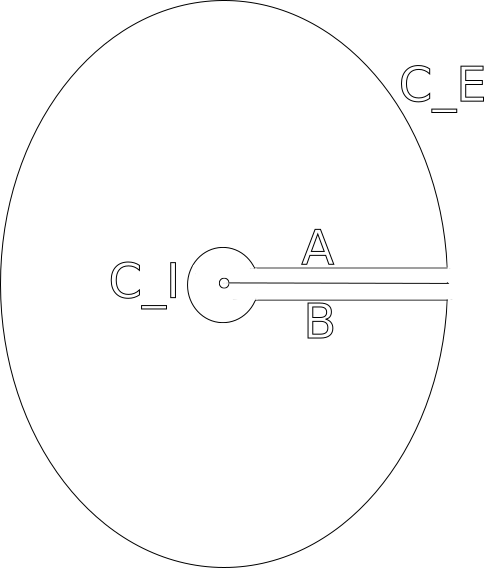
\includegraphics[width=0.3\textwidth]{img/fig3.png}
  \caption{Contorno en el que haremos la integral de este punto}
  \label{fig:fig3}
\end{figure}

Como se puede ver este contorno esta compuesto de cuatro trazos. $A$ es la integral que nos interesa, $B$ es la integral que nos intereza pero recorrida en el sentido opuesto. Por ultimo $C_I$ y $C_E$ son contornos que no van a aportarnos nada pues $\displaystyle\lim_{z \to \infty} \frac{1}{x^2} = 0$ y $\displaystyle\lim_{z \to 0} z^{p}\ln\left( z \right) = 0$.

Ahora bien, para el contorno $B$ podemos tomar que $z^{p} = x^{p}e^{2\pi i p}$ y $\ln\left( z \right) = \ln\left( x \right) + 2 \pi i$ por lo tanto esto queda:
\begin{align*}
  \int_{\infty}^{0} \frac{z^{p}\ln\left( z \right) }{z^2 + 1}dz &= - \int_0^{\infty} \frac{x^{p}e^{2\pi i p}\left[ \ln\left( z \right) + 2\pi i \right] }{x^2 + 1}dx \\
  &= -\left[ \int_{0}^{\infty}\frac{x^{p}e^{2\pi i p}\ln\left( x \right) }{x^2 + 1}  dx +  \int_{0}^{\infty} \frac{x^{p}e^{2 \pi i p}2 \pi i}{x^2 + 1} dx\right]\\
  &= -\left[ e^{2\pi i p}\int_{0}^{\infty}\frac{x^{p}\ln\left( x \right) }{x^2 + 1}dx + 2\pi i e^{2 \pi i p}\int_{0}^{\infty}\frac{x^{p}}{x^2 + 1} \right]  \\
  &= -e^{2\pi i p}I - 2\pi ie^{2 \pi i p}\int_{0}^{\infty} \frac{x^{p}}{x^2 + 1}dx
.\end{align*}

Esta ultima integral se hizo en el capitulo del libro. En particular, se hizo en el ejemplo $1.8.8$ y se hace de una manera muy similar a lo que estamos haciendo en este momento. Por lo tanto, no se hará en esta tarea y tendremos como uso el resultado de \[I = \frac{\pi\sin\left( \frac{p\pi}{2} \right) }{\sin\left( p\pi \right) } = \frac{\pi}{2\cos\left( \frac{p\pi}{2} \right) }.\]

Ahora, si juntamos todo tenemos: \[
  \oint_{C} \frac{z^{p}\ln\left( z \right) }{z^2 + 1}dz = I -e^{2\pi i p}I - 2\pi ie^{2 \pi i p}\frac{\pi}{2\cos\left( \frac{p\pi}{2} \right) } = I\left( 1 - e^{2\pi i p} \right) - \frac{\pi^2ie^{2\pi ip}}{\cos\left( \frac{p\pi}{2} \right) }
  .\] Ahora bien, note que: \[
  \oint_{C} \frac{z^{p}\ln\left( z \right) }{z^2 + 1} = \oint_{C} \frac{z^{p}\ln\left( z \right) }{\left( z + i \right) \left( z - i \right) }  
  .\] Por lo tanto, solo nos interesan los residuos en estos dos polos y sus residuos serian:
\begin{align*}
  Res_{z = i} \frac{z^{p}\ln\left( z \right) }{\left( z - i \right) \left( z + 1 \right) } &= \frac{e^{\pi i \frac{p}{2}}\left( \frac{\pi i}{2} \right) }{2i} \\
  Res_{z = i} \frac{z^{p}\ln\left( z \right) }{\left( z - i \right) \left( z + 1 \right) } &= \frac{e^{3\pi i \frac{p}{2}}\left( \frac{3\pi i}{2} \right) }{-2i} \\
  \oint_{C} \frac{z^{p}\ln\left( z \right) }{z^2 + 1} &= 2\pi i \sum Res \frac{z^{p}\ln\left( z \right) }{\left( z - i \right) \left( z + 1 \right) } \\
  &= 2\pi i \left[ \frac{e^{\pi i \frac{p}{2}}\left( \frac{\pi }{2} \right) }{2} - 3\frac{e^{3\pi i \frac{p}{2}}\left( \frac{\pi }{2} \right) }{2}\right]  \\
  &= \pi^2 i \left[ \frac{e^{\pi i \frac{p}{2}} - 3e^{3\pi i \frac{p}{2}}}{2} \right]  \\
  &= \frac{\pi^2 i}{2}\left[ e^{\pi i \frac{p}{2}} - 3e^{3\pi i \frac{p}{2}} \right]
.\end{align*}

Con lo cual tenemos la siguiente igualdad: \[
  \frac{\pi^2 i}{2}\left[ e^{\pi i \frac{p}{2}} - 3e^{3\pi i \frac{p}{2}} \right] =I\left( 1 - e^{2\pi i p} \right) - \frac{\pi^2ie^{2\pi ip}}{\cos\left( \frac{p\pi}{2} \right) }
  .\] Ahora desarrollamos con esto:
\begin{align*}
  \frac{\pi^2 i}{2}\left[ e^{\pi i \frac{p}{2}} - 3e^{3\pi i \frac{p}{2}} \right] &=I\left( 1 - e^{2\pi i p} \right) - \frac{\pi^2ie^{2\pi ip}}{\cos\left( \frac{p\pi}{2} \right) }\\
  I\left( 1 - e^{2\pi i p} \right) &= \frac{\pi^2 i}{2}\left[ e^{\pi i \frac{p}{2}} - 3e^{3\pi i \frac{p}{2}} \right] + \frac{\pi^2ie^{2\pi ip}}{\cos\left( \frac{p\pi}{2} \right) } \\
  &= \frac{\pi^2i}{2}\left[ e^{\pi i \frac{p}{2}} - 3e^{3\pi i \frac{p}{2}} + \frac{2e^{2 \pi i p}}{\cos\left( \frac{p\pi}{2} \right) } \right]  \\
  \text{Multiplicamos por }&-e^{-\pi i p}\\
  I\left( -e^{-\pi i p} + e^{i\pi p} \right)  &=  \frac{\pi^2i}{2}\left[ -e^{-\pi i \frac{p}{2}} + 3e^{\pi i \frac{p}{2}} - \frac{2e^{ \pi i p}}{\cos\left( \frac{p\pi}{2} \right) } \right]\\
  I\sin\left( p\pi \right) &= \frac{\pi i}{2}\left[ \frac{\sin^2\left( \frac{p \pi}{2} \right) }{\cos\left( \frac{p \pi}{2} \right) } \right]  \\
  I\left( 2\sin\left( \frac{p \pi}{2} \right) \cos\left( \frac{p \pi}{2} \right)  \right) &=  \frac{\pi i}{2}\left[ \frac{\sin^2\left( \frac{p \pi}{2} \right) }{\cos\left( \frac{p \pi}{2} \right) } \right]
.\end{align*}

Con lo cual llegamos al resultado deseado: \[
  I = \frac{\pi^2 \sin\left( \frac{p \pi}{2} \right)}{4 \cos^2\left( \frac{p\pi}{2} \right) }
  .\] 


\chapter{Pregunta 6: 11.8.22}

\qs{Pregunta 11.8.22}{
  Muestre que \[
    \displaystyle\int_0^{\infty} \frac{dx}{1 + x^{n}} = \frac{\frac{\pi}{n}}{\sin\left( \frac{\pi}{n} \right) }
    .\] 
  \textit{Pista:} Pruebe el contorno \ref{fig:11.8.22}, con $\theta = \frac{2\pi}{n}$

  \begin{figure}[H]
    \centering
    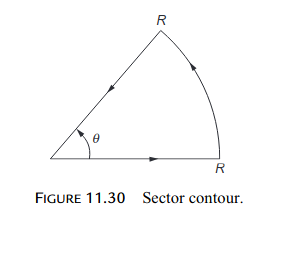
\includegraphics[width=0.4\textwidth]{img/fig1.png}
    \caption{Figura ayuda para el problema}
    \label{fig:11.8.22}
  \end{figure}

}

Para este caso tomando el contorno que nos dicen con $\theta = \frac{2\pi}{n}$ nos queda dividido en 3 contornos donde el semicirculo no aporta pues $\lim_{z \to \infty} \frac{1}{1 + z^{n}} = 0$. Ahora bien, tome en cuenta que podemos definir el valor que cambia si consideramos que esto queda básicamente como:
\begin{align*}
  \oint_{C} \frac{dz}{1 + z^{n}} &= \int_0^{\infty} \frac{dx}{1 + x^{n}} + \int_{\infty}^{0}e^{\frac{2\pi i}{n}} \frac{dx}{1 + x^{n}}\\ 
  &=  \int_0^{\infty} \frac{dx}{1 + x^{n}} - e^{\frac{2\pi i}{n}}\int_{0}^{\infty} \frac{dx}{1 + x^{n}}\\
  &= \left( 1 - e^{\frac{2\pi i}{n}} \right) \int_{0}^{\infty} \frac{dx}{1 + x^{n}} \\
.\end{align*}

Ahora bien, tenemos que la integral compleja encierra un polo simple en $z = e^{\frac{\pi i}{n}}$ por lo tanto podemos calcular su residuo con un limite:
\begin{align*}
  \lim_{z \to e^{\frac{\pi i}{n}}} \frac{z - e^{\frac{\pi i}{n}}}{1 + z^{n}} &= \lim_{z \to e^{\frac{\pi i}{n}}} \frac{1}{nz^{n - 1}} \\
  &= \lim_{z \to e^{\frac{\pi i}{n}}} \frac{z^{1 - n}}{n}  \\
  &= \frac{e^{\frac{\pi i}{n}\left( 1 - n \right) }}{n} \\
  &= \frac{e^{\frac{\pi i}{n}}e^{\pi i}}{n} \\
  &= \frac{e^{\frac{\pi i}{n}}}{n}
.\end{align*}

Con esto entonces:
\begin{align*}
  2\pi i\frac{e^{\frac{\pi i}{n}}}{n}&= \left( 1 - e^{\frac{2\pi i}{n}} \right) \int_{0}^{\infty} \frac{dx}{1 + x^{n}} \\
  \int_{0}^{\infty} \frac{dx}{1 + x^{n}} &= \frac{\pi}{n}\frac{2i e^{\frac{\pi i}{n}}}{\left( 1 - e^{\frac{2\pi i}{n}} \right)} \\
  &= \frac{\pi}{n\sin\left( \frac{\pi}{n} \right) }
.\end{align*}

\chapter{Pregunta 7: 11.8.27}

\qs{Pregunta 11.8.27}{
  Muestre que \[
    \displaystyle\int_{0}^{1} \frac{1}{\left( x^2 - x^{3} \right)^{\frac{1}{3}}}dx = \frac{2\pi}{\sqrt{3} }
    .\] 

  \textit{Pista:} Pruebe el contorno de la figura \ref{fig:11.8.27}

  \begin{figure}[H]
    \centering
    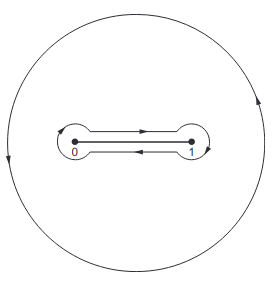
\includegraphics[width=0.3\textwidth]{img/fig2.png}
    \caption{Figura pregunta 11.8.27}
    \label{fig:11.8.27}
  \end{figure}
}

Para iniciar, note que podemos tomar: \[
  \oint_{C} \frac{dz}{z^{\frac{2}{3}}\left( 1 - z \right)^{\frac{1}{3}}} 
.\] 
\begin{enumerate}
  \item Linea arriba, de $0$ a $1$. Esta es básicamente la integral que queremos así que simplemente lo llamaremos $I$.
  \item Linea Abajo, de $1$ a $0$. Esto es en esencia el inverso de la integral que buscamos. Por lo tanto tomamos que $z^{\frac{2}{3}}= x^{\frac{2}{3}}$ y $\left( 1 - z \right)^{\frac{1}{3}} = e^{\frac{-2\pi i}{3}}\left( 1 - x \right)^{\frac{1}{3}}$. Por lo tanto, esto queda como: $-e^{\frac{2\pi i}{3}}I$
  \item Los dos círculos alrededor de $0$ y $1$ no aportan pues en ambos casos el limite se va a 0 y por tanto no aportan a la integral.
  \item En el circulo que rodea todo. En este caso el termino se vuelve $\frac{1}{\left( -1 \right)^{\frac{1}{3}}z}$ y debemos escoger una rama. Para hacerlo, note que en números grandes $z^{\frac{2}{3}} = x^{\frac{2}{3}}$, pero $\left( 1 - z \right)^{\frac{1}{3}} = \left| 1 - x \right|^{\frac{1}{3}}e^{\frac{-\pi i }{3}}$ por lo tanto, la integral se vuelve $\frac{1}{e^{\frac{-\pi i}{3}}z}$ con lo que se podría simplemente tomar como $e^{\frac{\pi i}{3}} \oint_{C_E} \frac{dz}{z} $ por lo que dado que que $C_E$ es una circunferencia el valor total seria $e^{\frac{\pi i}{3}}2\pi i$
\end{enumerate}

Ahora, ademas note que en este contorno no hay ningún polo dentro. Por lo tanto el resultado de la integral compleja es 0 y eso nos deja con la siguiente ecuación:
\begin{align*}
  I - e^{\frac{2\pi i}{3}}I + 2\pi ie^{\frac{\pi i}{3}} &= 0\\
  I \left( 1 - e^{\frac{2\pi i}{3}} \right) &= - 2\pi i e^{\frac{\pi i}{3}}\\
  I &= \frac{- 2\pi i e^{\frac{\pi i}{3}}}{\left( 1 - e^{\frac{2\pi i}{3}} \right)} \\
  &= -\frac{2i}{e^{-\frac{\pi i}{3}} \left( 1 - e^{\frac{2\pi i}{3}} \right) }\pi \\
  &= -\frac{2i}{e^{\frac{-\pi i}{3}} - e^{\frac{\pi i}{3}}}\pi \\
  &= \frac{2i}{e^{\frac{\pi i}{3}} - e^{\frac{-\pi i}{3}}} \\
  &= \frac{\pi}{\sin\left( \frac{\pi i}{3} \right) } \\
  &= \frac{\pi}{\frac{\sqrt{3} }{2}} \\
  &= \frac{2\pi}{\sqrt{3} }
.\end{align*}


\end{document}
